%! Author = Omar Iskandarani
%! Title = SST Photon and Laserbeam: Canon-consistent exposé (Dutch)
%! Date = Sept 4, 2025
%! Affiliation = Independent Researcher, Groningen, The Netherlands
%! License = To be set by PRB
%! ORCID = 0009-0006-1686-3961
%! DOI = 10.5281/zenodo.xxx
%========================================================================================
\newcommand{\paperdoi}{10.5281/zenodo.xxx}
%========================================================================================

%========================================================================================
% PACKAGES AND DOCUMENT CONFIGURATION
%========================================================================================
\documentclass[aps,prb,preprint,amsmath,amssymb]{revtex4-2} % switch to "reprint" for two-column look
\usepackage[utf8]{inputenc}
\usepackage[T1]{fontenc}
\usepackage{siunitx}
\usepackage{graphicx}
\usepackage{physics}
\usepackage{amsmath,amssymb,bm}
\usepackage[margin=1in]{geometry}
\usepackage[labelfont=bf]{caption}
\usepackage{tikz}
\usetikzlibrary{arrows.meta,positioning,fit}
% ---------- TikZ house styles (paste once) ----------
\tikzset{
    axis/.style   ={->,>=Latex,line width=0.6pt},
    thinline/.style={line width=0.6pt},
    bar/.style    ={draw,fill=gray!10,rounded corners=1pt},
    heater/.style ={draw,fill=red!15,rounded corners=1pt},
    sink/.style   ={draw,fill=blue!12,rounded corners=1pt},
    coilA/.style  ={thinline},
    coilB/.style  ={thinline,dashed},
    coilC/.style  ={thinline,dotted},
    lbl/.style    ={font=\footnotesize},
    note/.style   ={font=\scriptsize,align=center},
    box/.style    ={draw,rounded corners=2pt,fill=gray!8,inner sep=6pt},
    arr/.style    ={-Latex,line width=0.6pt},
}

\usepackage{pgfplots}\pgfplotsset{compat=1.18}
\usepackage[hidelinks]{hyperref}

% Safe \doi fallback (RevTeX usually defines \doi; this guards if not)
\providecommand{\doi}[1]{\href{https://doi.org/#1}{doi:\,#1}}

%-------------------------- SST minimal macro prelude (compile-safe) --------------------
% Vector swirl velocity + clock/vorticity symbols
\newcommand{\vswirl}{\mathbf{v}_{\!\mkern-2mu\scriptstyle\boldsymbol{\circlearrowleft}}}
\newcommand{\omegas}{\boldsymbol{\omega}_{\!\mkern-2mu\scriptstyle\boldsymbol{\circlearrowleft}}}
\newcommand{\rc}{r_c}
\newcommand{\rhoF}{\rho_{f}}
\newcommand{\rhoE}{\rho_{E}}
\newcommand{\rhoM}{\rho_{\!m}}
% \vswirl = 1.09384563e6 m s^-1 ; \rc = 1.40897017e-15 m ; \rhoF = 7.0e-7 kg m^-3
%----------------------------------------------------------------------------------------

\title{\textbf{Fotonen in Swirl--String Theory (SST):\\
kinematica op swirl-draden en het plotten van een laserstraal}}
\author{Omar Iskandarani}
\affiliation{Independent Researcher, Groningen, The Netherlands}
\thanks{ORCID: 0009-0006-1686-3961, DOI: \paperdoi}
\date{\today}

\begin{document}
    \maketitle

    \begin{abstract}
        We formuleren de foton als een eendimensionale, gesloten of open swirl-string met fase
        $\phi(\mathbf{x},t)$ die als helische voortplantingsmodus over de string loopt. Spin (circulaire polarisatie)
        komt overeen met de draairichting van de lokale swirl-clock; optisch impulsmoment (OAM) met topologische
        lading $\ell$ is de fasewinding in het transversale vlak. Voor laserstralen gebruiken we de
        (para\-xiale) Gaussische bundel en z'n Laguerre–Gauss-uitbreiding om intensiteit en fasevelden te plotten.
        Alle formules zijn SI-dimensioneel consistent en geijkt aan de SST-schaal $\Omega_0=\lVert\vswirl\rVert/\rc$.
    \end{abstract}

    \section{Kinematica: foton als helische modus op een swirl-string}
        Neem een string-centrumlijn $\mathbf{X}(s,t)$ met boogparameter $s$ en lokale tangent $\mathbf{t}$.
        Een foton wordt gemodelleerd als een \emph{travelling wave} op de string:
        \[
            \phi(\mathbf{x},t)=k z - \omega t + \ell\,\theta,\qquad k=\frac{2\pi}{\lambda}.
        \]
        waar $k=2\pi/\lambda$, $\omega=2\pi f$, en $(r,\theta,z)$ cil. coördinaten langs de voortplantingsas.
        De \emph{spin}/polarisatie is de draairichting van de lokale swirl (links/rechts), en de \emph{OAM}
        is de gehele winding $\ell\in\mathbb{Z}$ rond de bundelas \cite{Allen1992,Siegman1986}.

        \paragraph{SST-klok en energiedichtheid.}
            Een elementaire schaal is
            \[
                \Omega_0=\frac{\lVert\vswirl\rVert}{\rc}\quad [\si{ s^{-1} }].
            \]
            Dimensiecheck: $[\vswirl]=\si{m\,s^{-1}}$, $[\rc]=\si{m}$, dus $\Omega_0$ is een frequentie.
            Numeriek geeft dit de bekende Compton-schaal van het elektron; we gebruiken het als kalibratiepunt.

    \section{Energie, impuls en polarisatie}
    Voor een enkel foton geldt $E=\hbar\omega$ en $p=\hbar k$ (standaardveldentheorie).
    Binnen SST koppelen we de energie aan een effectieve lijnenergie van de string.
    Zonder verdere microdetailisering blijft de relationele kalender:
    \[
        \boxed{E=\hbar\omega,\quad \mathbf{p}=\hbar \mathbf{k},\quad
        \text{spin}\;S=\pm\hbar\ \leftrightarrow\ \text{swirl-clock links/rechts}}
    \]
    waarbij $+$ resp.\ $-$ overeenkomt met links- resp.\ rechtscirculaire polarisatie.

    \section{Laserstraalmodel: Gaussische bundel en LG-modi}
    Voor een paraxiale bundel met waist $w_0$ bij $z=0$ (\cite{Siegman1986}):
    \begin{align}
        w(z) &= w_0\sqrt{1+(z/z_R)^2},\qquad z_R=\frac{\pi w_0^2}{\lambda},\\
        R(z) &= z\!\left[1+\left(\frac{z_R}{z}\right)^2\right],\qquad
        \zeta(z)=\arctan\!\left(\frac{z}{z_R}\right).
    \end{align}
    De TEM$_{00}$ veldamplitude (scalar) is
    \[
        E_{00}(r,z)=E_0\frac{w_0}{w(z)}\exp\!\Big(-\frac{r^2}{w(z)^2}\Big)
        \exp\!\Big(i kz - i\omega t + i\frac{k r^2}{2R(z)} - i\,\zeta(z)\Big),
    \]
    De intensiteit is $I=\tfrac12\epsilon_0 c\,|E|^2$ (dimensie $\si{W\,m^{-2}}$).
    Laguerre–Gauss (LG) met OAM $\ell$ en radiale index $p$:
    \[
        E_{p}^{\ell}(r,\theta,z)=E_{00}\!\left(\frac{\sqrt{2}\,r}{w(z)}\right)^{|\ell|}
        L_p^{|\ell|}\!\!\left(\frac{2r^2}{w(z)^2}\right)e^{i\ell\theta}.
    \]
    Voor $\ell\neq 0$ is er een as-nul; het ringmaximum ligt bij
    $r_{\max}(z)=w(z)\sqrt{|\ell|/2}$.

    \section{Numeriek voorbeeld en figuren}
    Voorbeeldparameters: \(\lambda=\SI{632.8}{nm}\), \(w_0=\SI{1.0}{mm}\) $\Rightarrow$
    \(z_R=\pi w_0^2/\lambda=\SI{4.9646}{m}\) en
    bundeldivergentie \(\theta_{\mathrm{div}}=\lambda/(\pi w_0)=\SI{0.201}{mrad}\).

    \begin{figure}[h!]
        \centering
        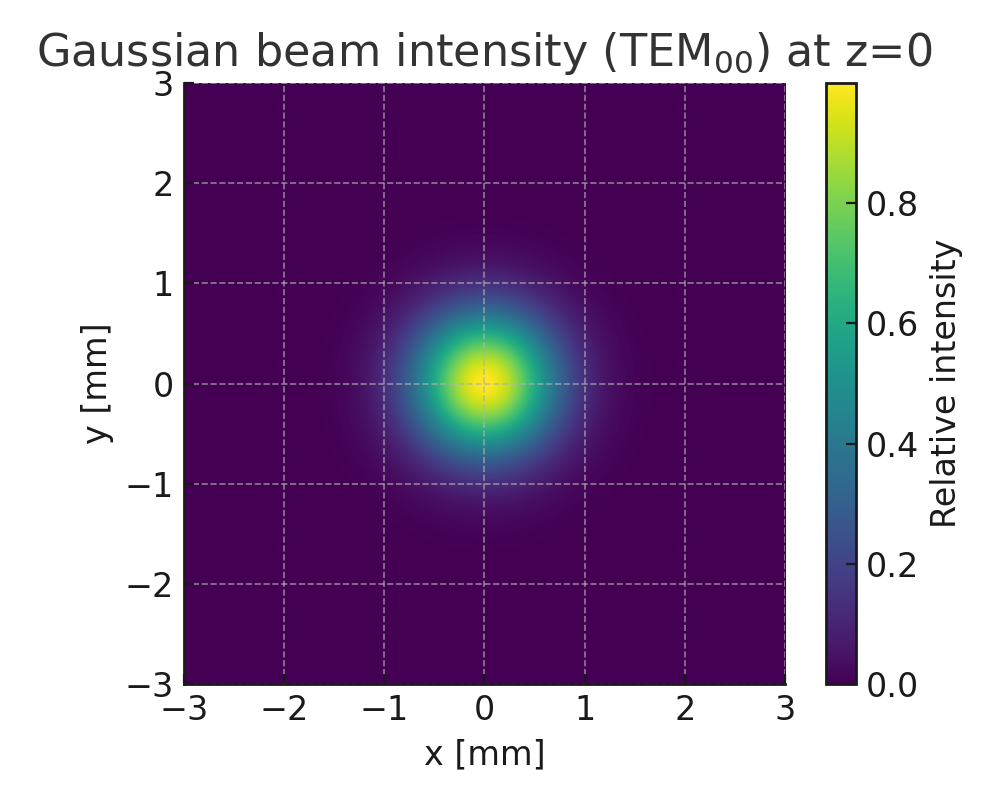
\includegraphics[width=0.78\linewidth]{gaussian_beam_intensity.png}
        \caption{\textbf{Gaussische intensiteit (TEM$_{00}$) in het $z{=}0$-vlak.}
        De kaart toont $I(r,0)\propto \exp(-2r^2/w_0^2)$ met een centrale piek en
        radiale Gauss-decay. Met $\lambda=\SI{632.8}{nm}$ en $w_0=\SI{1.0}{mm}$ is dit
        de bundelwaist. De dimensie van $I$ is $\si{W\,m^{-2}}$; hier wordt relatieve schaal weergegeven.}
        \label{fig:gauss}
    \end{figure}

    \begin{figure}[h!]
        \centering
        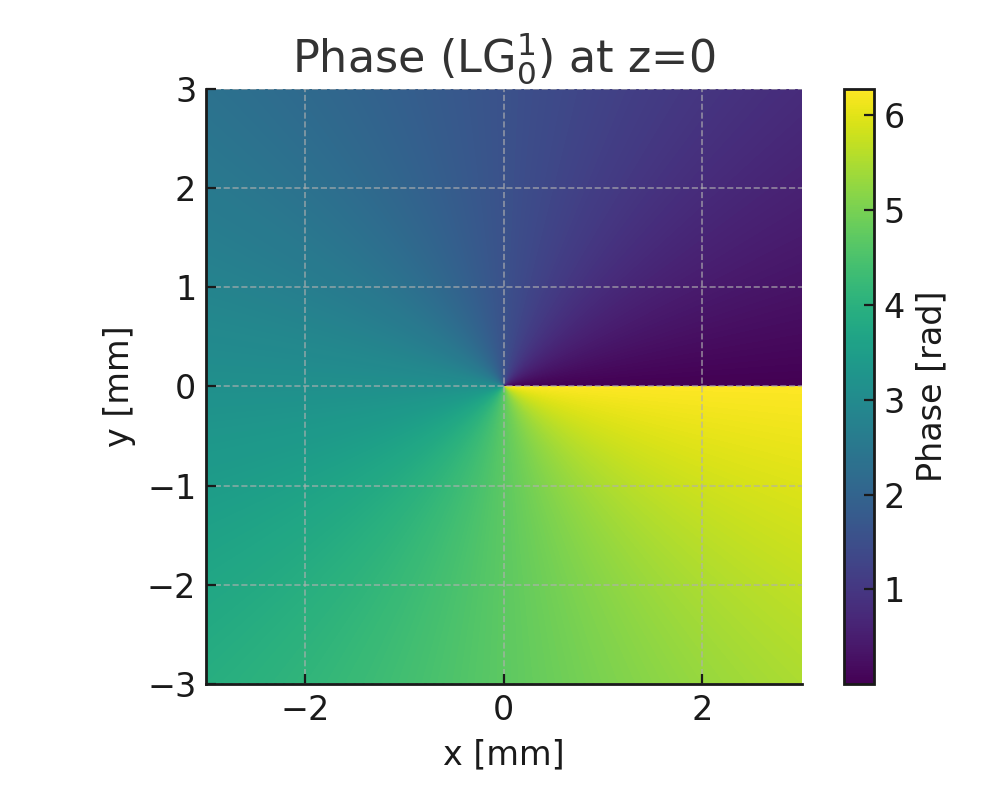
\includegraphics[width=0.78\linewidth]{lg_phase_l1.png}
        \caption{\textbf{Faseveld voor LG$_0^{1}$ met topologische lading $\ell{=}1$ in $z{=}0$.}
        De fase $\Phi(\theta)=\ell\,\theta$ windt $2\pi$ rond de as en heeft een singuliere kern
            (donkere ``vortex''): intensiteit nul op de as en een ringmaximum bij
            $r_{\max}(0)=w_0/\sqrt{2}=\SI{0.707}{mm}$. Dit visualiseert optisch impulsmoment (OAM).}
        \label{fig:lgphase}
    \end{figure}

    \begin{figure}[h!]
        \centering
        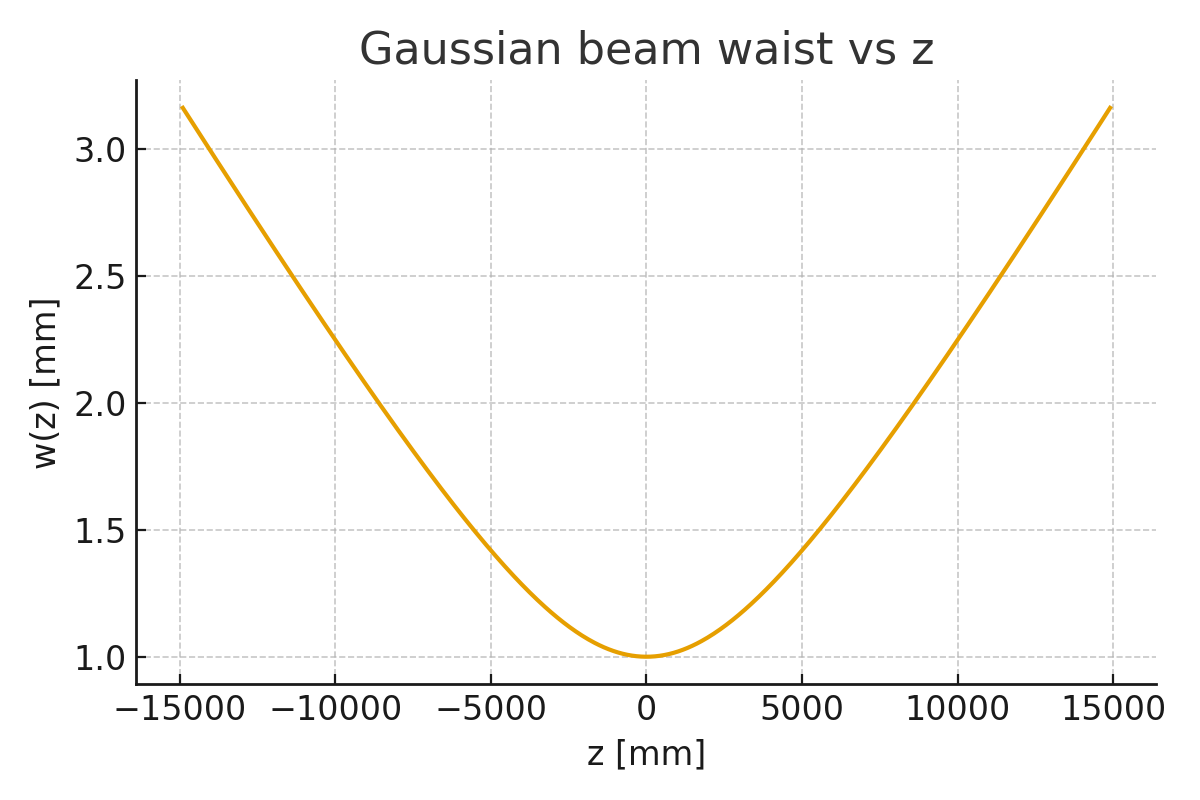
\includegraphics[width=0.78\linewidth]{beam_waist_vs_z.png}
        \caption{\textbf{Bundelwaist $w(z)$ versus $z$.}
        Voor $|z|\ll z_R$ blijft de bundel smal; voor $|z|\gg z_R$ groeit $w(z)\approx |z|\theta_{\mathrm{div}}$
            met $\theta_{\mathrm{div}}=\lambda/(\pi w_0)$. Het Rayleigh-bereik $z_R=\SI{4.9646}{m}$
            markeert de overgang tussen nabij- en ver-veld.}
        \label{fig:waist}
    \end{figure}

    \paragraph{Leeshulp.}
        Fig.~\ref{fig:gauss} toont de TEM$_{00}$-intensiteit op de waist ($z=0$).
        Fig.~\ref{fig:lgphase} laat de $2\pi$-fasewinding voor $\ell=1$ zien (OAM, nul op de as).
        Fig.~\ref{fig:waist} bevestigt de bekende schaling $w(z)$ en de divergente limiet.

        Bekende limieten: $w(0)=w_0$, veraf $z\gg z_R$ geeft openingshoek $\theta_{\rm div}\!=\!\lambda/(\pi w_0)$,
        en voor $\ell\neq 0$ is er een as-nul met ringmaximum $r_{\max}(z)=w(z)\sqrt{|\ell|/2}$ \cite{Allen1992,Berry2001}.

    \section{Plotrecept (algoritme)}
    \begin{enumerate}
        \item Kies \(\lambda\), \(w_0\); bereken \(z_R=\pi w_0^2/\lambda\).
        \item Definieer een 2D raster in het $z=0$ vlak; compute \(I(r,0)\propto e^{-2r^2/w_0^2}\) (TEM$_{00}$).
        \item Voor OAM, neem fase \(\Phi=\ell\,\theta\) en (optioneel) de LG-omhulling.
        \item Voor doorsnede langs $z$: plot \(w(z)\) en (desgewenst) \(r_{\max}(z)\).
    \end{enumerate}

    \section{Numeriek voorbeeld (HeNe-achtig)}
    Neem \(\lambda=\SI{632.8}{nm}\), \(w_0=\SI{1.0}{mm}\).
    Dan \(z_R=\SI{4.9646}{m}\) en \(\theta_{\rm div}=\lambda/(\pi w_0)=\SI{0.201}{mrad}\).
    Voor \(\ell=1\) geldt \(r_{\max}(0)=w_0/\sqrt{2}=\SI{0.707}{mm}\).

    \section{Voorspellingen (falsifieerbaar) en randgevallen}
    \textbf{P1 (spin↔swirl-clock).} Helicity van polarisatie valt 1-op-1 samen met de draairichting van de lokale swirl-clock;
    spin–to–orbital conversie bij sterke focus levert stapjes in $\ell$ (controleer via interferentie-forks \cite{Berry2001}).
    \textbf{P2 (OAM-ring).} De nul op de as en ringradius \(r_{\max}\) volgen exact de LG-schaal;
    afwijkingen bij extreme focus (niet-paraxiaal) voorspellen meetbare fasemodulaties.
    \textbf{Randgevallen.} Niet-paraxiaal (\(w_0\!\sim\!\lambda\)), dispersieve media, en nabij-veld van structuren
    (lokaal niet-Gaussiaans) vragen om volledige (vectoriële) oplossingsvormen.

    \paragraph{Analogie (10-jarige).}
        Een foton is als een piepkleine kurkentrekker-rimpel die langs een onzichtbaar touwtje vooruit schroeft:
        linksom of rechtsom bepaalt de polarisatie; met extra draai per rondje krijg je OAM-ringen.


        \bibliographystyle{unsrt}
        \begin{thebibliography}{9}
            \bibitem{Siegman1986} A.~E.~Siegman, \emph{Lasers}, University Science Books (1986).
            \bibitem{Allen1992} L.~Allen \emph{et al.}, Phys. Rev. A \textbf{45}, 8185 (1992).
            \bibitem{Berry2001} M.~V.~Berry, J. Opt. A \textbf{6}, 259 (2004).
        \end{thebibliography}

\end{document}